\begin{figure}[!htbp]
    \begin{minipage}{0.55\textwidth}
        \centering
        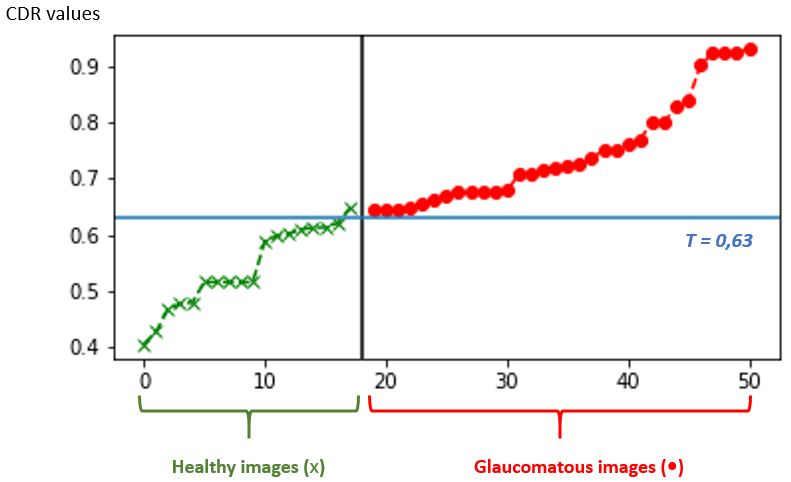
\includegraphics[width=0.9\textwidth]{Images/Results/Classification/ratio_legende.jpg}
        \captionof{figure}{\label{courbe_aire}CDR value for each retinal image, from healthy (green) class and glaucomatous (red) class (along x-axis: fifty annotated images from DRISHTI-GS1, along y-axis: CDR values (between 0 and 1)). The threshold value T = 0.63 is plotted in blue line along y-axis.}
    \end{minipage}
    \hfill
    \begin{minipage}{0.4\textwidth}
       \centering
       \begin{tabular}{|c|c|c|c|}
        \hline
        \multicolumn{2}{|c|}{Healthy class} & \multicolumn{2}{c|}{Glaucomatous class} \\
        \hline
        Mean & Standard & Mean & Standard  \\
        $\bar{m_H}$ & deviation & $\bar{m_G}$ & deviation \\
        {} & $\sigma_{H}$ & {} & $\sigma_{G}$ \\
        \hline
        0.541 & 0.07 & 0.74 & 0.09 \\
        \hline
        \end{tabular}
        \captionof{table}{\label{tableau_cdr_values}CDR mean and standard deviation values for healthy and glaucomatous classes.}
    \end{minipage}
\end{figure}